
\chapter{Security
}\label{kap:security}

\section{Security and Design}

Here is a data flow diagram to help identify a flow of data and interactions between components in the application:

\begin{figure}[H]
   \centering
   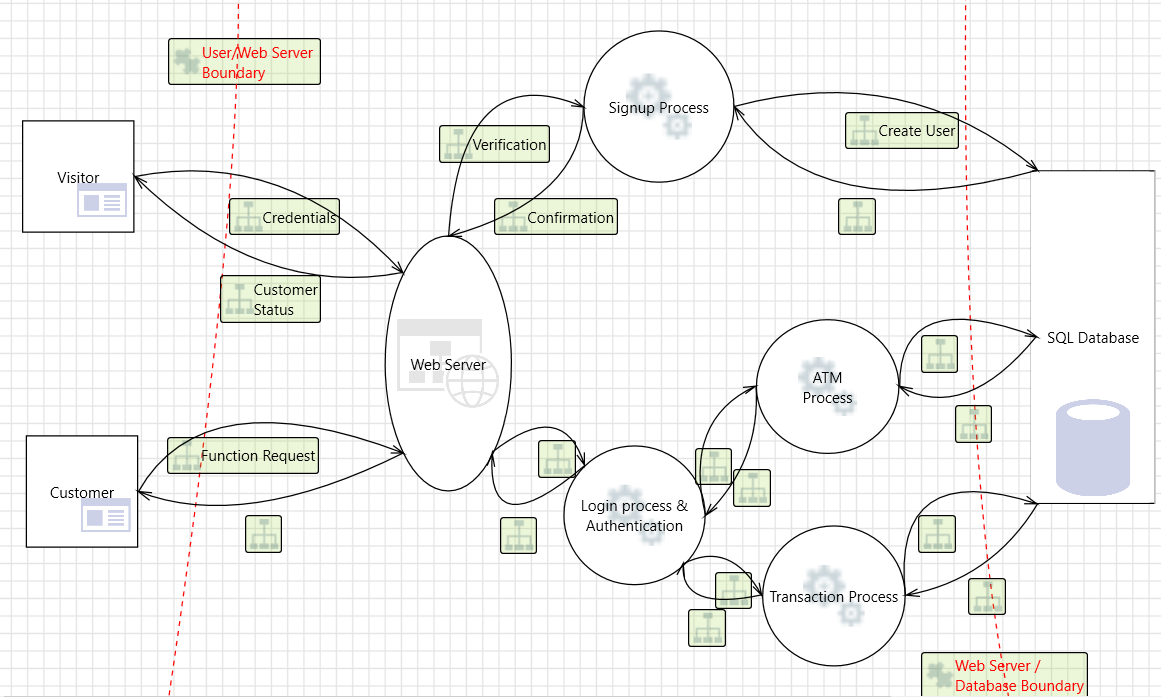
\includegraphics[width=\textwidth]{pics/pic4 Data Flow.PNG}
   \caption{Data flow}
   \label{fig:cha2fig1dataflow}
\end{figure}

Some possible threats that we could identify by looking at the system model are:
\begin{itemize}
   \item Spoofing
   \begin{itemize}
      \item Credential stuffing (attacker having list of valid usernames and passwords)
      \item Brute force authentication
      \item Evading the authentication system and exploiting session management
      \item Cross-Site Request Forgery
      \item Missing session timeouts 
  \end{itemize}
  \item Tampering
  \begin{itemize}
     \item Improper input validation
     \item SQL injection
     \item XML injection
     \item Forcefully browsing to authenticated pages 
     \item tampering with URL to avoid authentication checks
   \end{itemize}
   \item Repudiation
   \begin{itemize}
    \item  Lack of monitoring (performing unauthorized operation without the ability to be traced or detected)
   \end{itemize}
   \item Information disclosure
   \begin{itemize}
     \item Unauthorized access to database
     \item Capturing non-encrypted data
     \item Access to weakly encrypted content
   \end{itemize}
\end{itemize}

In next sections we will show the basics of how our website is structured in the code and how our features are implemented within our website. Lastly we will look at how to mitigate some of these threats mentioned above both in chapter 1 but also in chapter 2. % TODO, ref chapters

\subsection{Design choices}

We “deny by default” all but essential intranet traffic, the only way to have a read/write connection with our database, is to log in, or sign up.
Otherwise, the site is in a "special" read-only status, where you can only view the public html, and get no data from the database. Like most, if not all, secure websites.

We decided that it's better design-wise to have one "master" class for transactions, and not to have a "balance" value in our database table, it comes with a number of advantages:
\begin{itemize}
    \item It's easier to keep track with abnormalities, if anything fishy is going on, our system will show us why and how.
    \item It's much harder to directly change the balance value in the database, since it's not stored in one place, and all the transactions should be read-only once verified and validated.
    \item It's an easier system to manage, than having two separate data classes for normal transaction, and one-user transactions (ATM).
\end{itemize}

\Que{Why can from and out money values be null?}
\Ans{Because ATM process allows for putting in money, where there is not user/user account to get money from}
\Que{Why are we saving money value data in a string?}
\Ans{With some research, there were two options of saving money amounts. Either with a non-fixed point decimal, or a long string. Since SQL\textunderscore Alchemy doesn't support decimals too well.We decided to go with a very long string instead, that way we can have perfect precision, and support very large numbers as well.}

\section{How features are implemented}

\subsection{Getting user input}

WTForms extension is used to gather and validate input from users. Depending on the need, built-in or custom validators are used, unfortunately it can be easily bypassed so this is our front-end checks. We implemented it by  creating a Flask form class which is shown in the picture below and this method is used for every input we get from a user. For example, sign-up transactions etc. 

\begin{python}
class LoginForm(FlaskForm):
   email = StringField(label='Email', validators=[Email()])
   password = PasswordField(label='Password',
                            validators=[DataRequired(),
                            Length(min=1, max=100,
                            message="Password must be between"
                           +"7 and 100 characters!")])
   
   OTP = IntegerField(label="Your one time password",
                      validators=[DataRequired()])

   recaptcha = RecaptchaField()

   submit = SubmitField(label='Log in')
\end{python}

We validate the user input on our back-end as well using various function to check if it contains any illegal characters. More on this in the next chapter.  %TODO REF

\subsection{Creating user}

When the signup form is sent, the input is validated both within WTForms and on backend, then a check is made to see if a user with a given name or email already exists. If not - then the given password is hashed and user data is sent to the database and saved. The application then redirects you to the homepage. We also logs this info in our log database model. If something goes wrong during the process, a red error message will appear.

\begin{figure}[H]
    \centering
    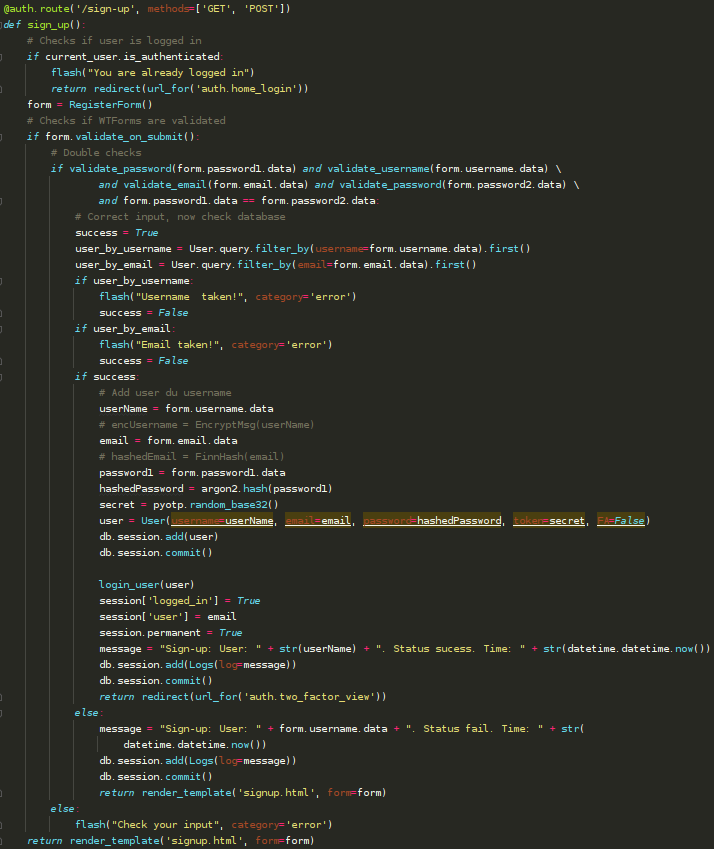
\includegraphics[width=\textwidth]{pics/pic7 signup.png}
    \caption{Sign up backend code}
    \label{fig:cha2fig2signupcode}
\end{figure}

Argon2 function is being used to hash passwords.

\subsection{Login process/Session management}

When the login form is sent, the input is also validated both front-end and backend. Then the database is searched for a user with a given email and given password is compared with hashed database password. It also checks for reCAPTCHA and the OTP (one-time-password) is correct. If everything is okay, the app redirects the user to his homepage. If something goes wrong during the process, a red error message will appear.

\begin{figure}[H]
    \centering
    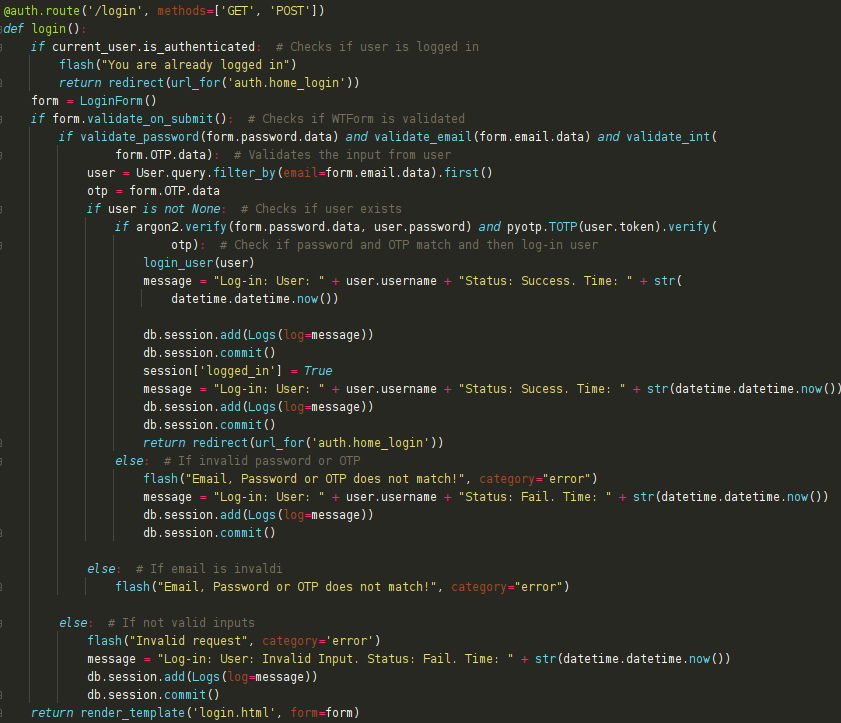
\includegraphics[width=\textwidth]{pics/pic8 login.png}
    \caption{Login backend code}
    \label{fig:cha2fig3logincode}
\end{figure}

Furthermore a user can log out simply by clicking on the logout button in the navigation bar, and gets redirected to the log-in page. 

The application uses the Flask-Login extension for session management. It allows us to restrict some pages to be visible only for logged-in users, but we will go deeper into the security of this in the next chapter. %TODO REF

\begin{figure}[H]
   \centering
   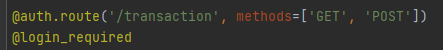
\includegraphics[width=\textwidth]{pics/pic9.1 loginrequired.PNG}
   \caption{Login required}
   \label{fig:cha2fig3loginrequired}
\end{figure}

\begin{figure}[H]
   \centering
   
\includegraphics[width=\textwidth]{pics/pic9.2 need to log in.PNG}
   \caption{No access}
   \label{fig:cha2fig4noaccess}
\end{figure}

\subsection{ATM and Transaction}

These services first validate data both front-end and back-end. Then authenticate given data to check if said username exists, valid amount etc. It also check for reCAPTCHA and OTP. If everything checks out, a transaction is made. If something goes wrong during the process, a red error message will appear. 

\subsection{Database}

Flask-sqlalchemy extension provides support for SQLALchemy. We use three database models – user, transaction and Logs. The user stores the user information, like username, email, password, id, token(used for 2FA) and FA check (whether they have already accesses QR-code page). The password is stored in the database using argon2 hash. We will discuss our approach on why we chose this algorithm in the next chapter. 

In our transaction model we save the id of the transaction, from\_user, to\_user, in and out money and a message. As you have seen we don’t store the account balance in the database as a security measures and to get as close to the real world as possible. We simply use a for loop to go through each transaction for that given user. The implementation looks like this:

\begin{python}
class Transaction(UserMixin, db.Model):
   transaction_id = db.Column(db.Integer, primary_key=True)
   from_user_id = db.Column(db.Text, nullable=True)  
   out_money = db.Column(db.Text, nullable=True)
   to_user_id = db.Column(db.Text) 
   in_money = db.Column(db.Text)
   message = db.Column(db.String(120))
\end{python}

Lastly we have another database model called logs. This simply stores the id of the log and the log message, which contains the action made, user (if any), success or fail and what time it was logged/happened. We store both success made by a user and failures. 

\begin{python}
class Logs(db.Model):
    log_id = db.Column(db.Integer, primary_key=True)
    log = db.Column(db.Text)
\end{python}
